\begin{figure}[!h]
  \centerline{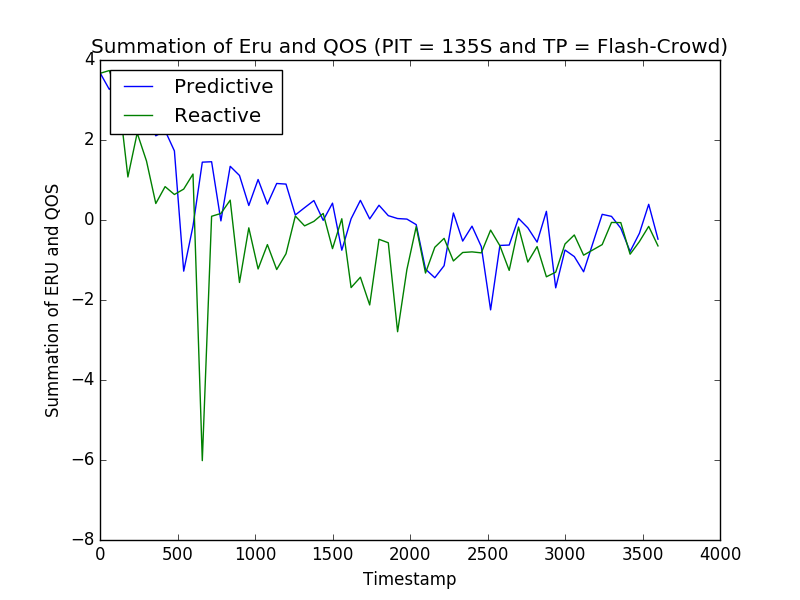
\includegraphics[scale=.75]{graph_135s_flash-crowd.png}}
  \caption{The graph for 135s, flash-crowd}
  \label{fig:135s-flash-crowd}
\end{figure}

\begin{table}[htbp]
  \centering
  \caption{Difference in Predictive and Reactive Auto-scaling for 135s, flash-crowd}
  \label{tab:135s-flash-crowd}
\begin{tabular}{l c}\hline\hline
    \multicolumn{1}{c}{\textbf{Measure}} & \textbf{Value} \\ \hline
     p-value & 0.549 \\
     z-score & -.124 \\
     std\_dev & 1.056 \\
     mean & -.130
  \end{tabular}
\end{table}

Figure \ref{fig:135s-flash-crowd} contains a graph
showing predictive and reactive auto-scaling's different
summations of efficient resource utilization and quality of service over the
course of the forty minute trial. Additionally, Table
\ref{tab:135s-flash-crowd} shows summary statistics for predictive
auto-scaling's summation of ERU and QOS minus reactive auto-scaling's summation
of ERU and QOS for corresponding intervals.

A similar process as occurs with respect to increase-decrease can be seen in the
flash-crowd traffic pattern. We are unable to reject our null hypothesis in
favor of the alternative hypothesis. Yet, once again there is insight to be
gained based on the comparative performance of predictive and reactive
auto-scaling. Our predictive auto-scaling implementation performs
very well initially, as can be seen in its first pronounced spike. However, soon
after, there is a substantial downward spike during the interval when Kubernetes
forbids auto-scaling to prevent thrashing. After that threshold interval is
passed, our predictive auto-scaling begins to perform better than reactive
auto-scaling, which is entering its own period at which it is unable to scale
because it is in the threshold. Given similar patterns of Kubernetes behavior
with respect to the increase-decrease and flash-crowd traffic pattern, we can
comment on the general times at which predictive auto-scaling outperforms
reactive auto-scaling and the general times at which the converse is true.
